% Options for packages loaded elsewhere
\PassOptionsToPackage{unicode}{hyperref}
\PassOptionsToPackage{hyphens}{url}
\PassOptionsToPackage{dvipsnames,svgnames,x11names}{xcolor}
%
\documentclass[
  letterpaper,
  DIV=11,
  numbers=noendperiod]{scrreprt}

\usepackage{amsmath,amssymb}
\usepackage{iftex}
\ifPDFTeX
  \usepackage[T1]{fontenc}
  \usepackage[utf8]{inputenc}
  \usepackage{textcomp} % provide euro and other symbols
\else % if luatex or xetex
  \usepackage{unicode-math}
  \defaultfontfeatures{Scale=MatchLowercase}
  \defaultfontfeatures[\rmfamily]{Ligatures=TeX,Scale=1}
\fi
\usepackage{lmodern}
\ifPDFTeX\else  
    % xetex/luatex font selection
\fi
% Use upquote if available, for straight quotes in verbatim environments
\IfFileExists{upquote.sty}{\usepackage{upquote}}{}
\IfFileExists{microtype.sty}{% use microtype if available
  \usepackage[]{microtype}
  \UseMicrotypeSet[protrusion]{basicmath} % disable protrusion for tt fonts
}{}
\makeatletter
\@ifundefined{KOMAClassName}{% if non-KOMA class
  \IfFileExists{parskip.sty}{%
    \usepackage{parskip}
  }{% else
    \setlength{\parindent}{0pt}
    \setlength{\parskip}{6pt plus 2pt minus 1pt}}
}{% if KOMA class
  \KOMAoptions{parskip=half}}
\makeatother
\usepackage{xcolor}
\usepackage[heightrounded]{geometry}
\setlength{\emergencystretch}{3em} % prevent overfull lines
\setcounter{secnumdepth}{-\maxdimen} % remove section numbering
% Make \paragraph and \subparagraph free-standing
\ifx\paragraph\undefined\else
  \let\oldparagraph\paragraph
  \renewcommand{\paragraph}[1]{\oldparagraph{#1}\mbox{}}
\fi
\ifx\subparagraph\undefined\else
  \let\oldsubparagraph\subparagraph
  \renewcommand{\subparagraph}[1]{\oldsubparagraph{#1}\mbox{}}
\fi

\usepackage{color}
\usepackage{fancyvrb}
\newcommand{\VerbBar}{|}
\newcommand{\VERB}{\Verb[commandchars=\\\{\}]}
\DefineVerbatimEnvironment{Highlighting}{Verbatim}{commandchars=\\\{\}}
% Add ',fontsize=\small' for more characters per line
\newenvironment{Shaded}{}{}
\newcommand{\AlertTok}[1]{\textcolor[rgb]{1.00,0.33,0.33}{\textbf{#1}}}
\newcommand{\AnnotationTok}[1]{\textcolor[rgb]{0.42,0.45,0.49}{#1}}
\newcommand{\AttributeTok}[1]{\textcolor[rgb]{0.84,0.23,0.29}{#1}}
\newcommand{\BaseNTok}[1]{\textcolor[rgb]{0.00,0.36,0.77}{#1}}
\newcommand{\BuiltInTok}[1]{\textcolor[rgb]{0.84,0.23,0.29}{#1}}
\newcommand{\CharTok}[1]{\textcolor[rgb]{0.01,0.18,0.38}{#1}}
\newcommand{\CommentTok}[1]{\textcolor[rgb]{0.42,0.45,0.49}{#1}}
\newcommand{\CommentVarTok}[1]{\textcolor[rgb]{0.42,0.45,0.49}{#1}}
\newcommand{\ConstantTok}[1]{\textcolor[rgb]{0.00,0.36,0.77}{#1}}
\newcommand{\ControlFlowTok}[1]{\textcolor[rgb]{0.84,0.23,0.29}{#1}}
\newcommand{\DataTypeTok}[1]{\textcolor[rgb]{0.84,0.23,0.29}{#1}}
\newcommand{\DecValTok}[1]{\textcolor[rgb]{0.00,0.36,0.77}{#1}}
\newcommand{\DocumentationTok}[1]{\textcolor[rgb]{0.42,0.45,0.49}{#1}}
\newcommand{\ErrorTok}[1]{\textcolor[rgb]{1.00,0.33,0.33}{\underline{#1}}}
\newcommand{\ExtensionTok}[1]{\textcolor[rgb]{0.84,0.23,0.29}{\textbf{#1}}}
\newcommand{\FloatTok}[1]{\textcolor[rgb]{0.00,0.36,0.77}{#1}}
\newcommand{\FunctionTok}[1]{\textcolor[rgb]{0.44,0.26,0.76}{#1}}
\newcommand{\ImportTok}[1]{\textcolor[rgb]{0.01,0.18,0.38}{#1}}
\newcommand{\InformationTok}[1]{\textcolor[rgb]{0.42,0.45,0.49}{#1}}
\newcommand{\KeywordTok}[1]{\textcolor[rgb]{0.84,0.23,0.29}{#1}}
\newcommand{\NormalTok}[1]{\textcolor[rgb]{0.14,0.16,0.18}{#1}}
\newcommand{\OperatorTok}[1]{\textcolor[rgb]{0.14,0.16,0.18}{#1}}
\newcommand{\OtherTok}[1]{\textcolor[rgb]{0.44,0.26,0.76}{#1}}
\newcommand{\PreprocessorTok}[1]{\textcolor[rgb]{0.84,0.23,0.29}{#1}}
\newcommand{\RegionMarkerTok}[1]{\textcolor[rgb]{0.42,0.45,0.49}{#1}}
\newcommand{\SpecialCharTok}[1]{\textcolor[rgb]{0.00,0.36,0.77}{#1}}
\newcommand{\SpecialStringTok}[1]{\textcolor[rgb]{0.01,0.18,0.38}{#1}}
\newcommand{\StringTok}[1]{\textcolor[rgb]{0.01,0.18,0.38}{#1}}
\newcommand{\VariableTok}[1]{\textcolor[rgb]{0.89,0.38,0.04}{#1}}
\newcommand{\VerbatimStringTok}[1]{\textcolor[rgb]{0.01,0.18,0.38}{#1}}
\newcommand{\WarningTok}[1]{\textcolor[rgb]{1.00,0.33,0.33}{#1}}

\providecommand{\tightlist}{%
  \setlength{\itemsep}{0pt}\setlength{\parskip}{0pt}}\usepackage{longtable,booktabs,array}
\usepackage{calc} % for calculating minipage widths
% Correct order of tables after \paragraph or \subparagraph
\usepackage{etoolbox}
\makeatletter
\patchcmd\longtable{\par}{\if@noskipsec\mbox{}\fi\par}{}{}
\makeatother
% Allow footnotes in longtable head/foot
\IfFileExists{footnotehyper.sty}{\usepackage{footnotehyper}}{\usepackage{footnote}}
\makesavenoteenv{longtable}
\usepackage{graphicx}
\makeatletter
\def\maxwidth{\ifdim\Gin@nat@width>\linewidth\linewidth\else\Gin@nat@width\fi}
\def\maxheight{\ifdim\Gin@nat@height>\textheight\textheight\else\Gin@nat@height\fi}
\makeatother
% Scale images if necessary, so that they will not overflow the page
% margins by default, and it is still possible to overwrite the defaults
% using explicit options in \includegraphics[width, height, ...]{}
\setkeys{Gin}{width=\maxwidth,height=\maxheight,keepaspectratio}
% Set default figure placement to htbp
\makeatletter
\def\fps@figure{htbp}
\makeatother

\usepackage{fvextra}
\DefineVerbatimEnvironment{Highlighting}{Verbatim}{breaklines,commandchars=\\\{\}}
\KOMAoption{captions}{tableheading}
\makeatletter
\@ifpackageloaded{tcolorbox}{}{\usepackage[skins,breakable]{tcolorbox}}
\@ifpackageloaded{fontawesome5}{}{\usepackage{fontawesome5}}
\definecolor{quarto-callout-color}{HTML}{909090}
\definecolor{quarto-callout-note-color}{HTML}{0758E5}
\definecolor{quarto-callout-important-color}{HTML}{CC1914}
\definecolor{quarto-callout-warning-color}{HTML}{EB9113}
\definecolor{quarto-callout-tip-color}{HTML}{00A047}
\definecolor{quarto-callout-caution-color}{HTML}{FC5300}
\definecolor{quarto-callout-color-frame}{HTML}{acacac}
\definecolor{quarto-callout-note-color-frame}{HTML}{4582ec}
\definecolor{quarto-callout-important-color-frame}{HTML}{d9534f}
\definecolor{quarto-callout-warning-color-frame}{HTML}{f0ad4e}
\definecolor{quarto-callout-tip-color-frame}{HTML}{02b875}
\definecolor{quarto-callout-caution-color-frame}{HTML}{fd7e14}
\makeatother
\makeatletter
\@ifpackageloaded{caption}{}{\usepackage{caption}}
\AtBeginDocument{%
\ifdefined\contentsname
  \renewcommand*\contentsname{Table of contents}
\else
  \newcommand\contentsname{Table of contents}
\fi
\ifdefined\listfigurename
  \renewcommand*\listfigurename{List of Figures}
\else
  \newcommand\listfigurename{List of Figures}
\fi
\ifdefined\listtablename
  \renewcommand*\listtablename{List of Tables}
\else
  \newcommand\listtablename{List of Tables}
\fi
\ifdefined\figurename
  \renewcommand*\figurename{Figure}
\else
  \newcommand\figurename{Figure}
\fi
\ifdefined\tablename
  \renewcommand*\tablename{Table}
\else
  \newcommand\tablename{Table}
\fi
}
\@ifpackageloaded{float}{}{\usepackage{float}}
\floatstyle{ruled}
\@ifundefined{c@chapter}{\newfloat{codelisting}{h}{lop}}{\newfloat{codelisting}{h}{lop}[chapter]}
\floatname{codelisting}{Listing}
\newcommand*\listoflistings{\listof{codelisting}{List of Listings}}
\makeatother
\makeatletter
\makeatother
\makeatletter
\@ifpackageloaded{caption}{}{\usepackage{caption}}
\@ifpackageloaded{subcaption}{}{\usepackage{subcaption}}
\makeatother
\makeatletter
\@ifpackageloaded{tcolorbox}{}{\usepackage[skins,breakable]{tcolorbox}}
\makeatother
\makeatletter
\@ifundefined{shadecolor}{\definecolor{shadecolor}{HTML}{31BAE9}}{}
\makeatother
\makeatletter
\makeatother
\makeatletter
\ifdefined\Shaded\renewenvironment{Shaded}{\begin{tcolorbox}[sharp corners, boxrule=0pt, interior hidden, borderline west={3pt}{0pt}{shadecolor}, breakable, enhanced, frame hidden]}{\end{tcolorbox}}\fi
\makeatother
\ifLuaTeX
  \usepackage{selnolig}  % disable illegal ligatures
\fi
\usepackage{bookmark}

\IfFileExists{xurl.sty}{\usepackage{xurl}}{} % add URL line breaks if available
\urlstyle{same} % disable monospaced font for URLs
\hypersetup{
  colorlinks=true,
  linkcolor={blue},
  filecolor={Maroon},
  citecolor={Blue},
  urlcolor={Blue},
  pdfcreator={LaTeX via pandoc}}

\author{}
\date{}

\begin{document}

\RecustomVerbatimEnvironment{verbatim}{Verbatim}{
  showspaces = false,
  showtabs = false,
  breaksymbolleft={},
  breaklines
}

\renewcommand*\contentsname{Table of contents}
{
\hypersetup{linkcolor=}
\setcounter{tocdepth}{2}
\tableofcontents
}
\chapter{Using an HPC}\label{using-an-hpc}

Now, that you are familiar more familiar with the cli, let's get used to
working on an HPC by first login into Crunchomics, uploading our
sequencing data an run some software to check the quality of our reads.

For people following this tutorial outside of UvA:

\begin{itemize}
\tightlist
\item
  If you have access to an HPC using SLURM you still follow the tutorial
\item
  If you do not have access to an HPC but are interested in how to
  install and run software that can be used to analyse sequencing data,
  you still might want to check out the steps run below. The dataset is
  very small and all analyses can be run on a desktop computer
\end{itemize}

\section{\texorpdfstring{\texttt{ssh}: Connecting to a
sever}{ssh: Connecting to a sever}}\label{ssh-connecting-to-a-sever}

\textbf{SSH} (Secure Shell) is a network protocol that enables secure
remote connections between two systems. The general \texttt{ssh} command
that you can use to login into any HPC looks as follows:

\begin{Shaded}
\begin{Highlighting}[]
\FunctionTok{ssh} \AttributeTok{{-}X}\NormalTok{ username@server}
\end{Highlighting}
\end{Shaded}

Options:

\begin{itemize}
\tightlist
\item
  \texttt{-X} option enables untrusted X11 forwarding in SSH. Untrusted
  means = your local client sends a command to the remote machine and
  receives the graphical output. Put simply this option enables us to
  run graphical applications on a remote server and this for example
  allows us to view a pdf.
\end{itemize}

If you have access to and want to connect to Crunchomics you would edit
the command above to look like this:

\begin{Shaded}
\begin{Highlighting}[]
\FunctionTok{ssh} \AttributeTok{{-}X}\NormalTok{ uvanetid@omics{-}h0.science.uva.nl}
\end{Highlighting}
\end{Shaded}

\begin{tcolorbox}[enhanced jigsaw, colframe=quarto-callout-important-color-frame, breakable, opacityback=0, toptitle=1mm, left=2mm, coltitle=black, colbacktitle=quarto-callout-important-color!10!white, title=\textcolor{quarto-callout-important-color}{\faExclamation}\hspace{0.5em}{Important}, rightrule=.15mm, bottomtitle=1mm, titlerule=0mm, colback=white, arc=.35mm, toprule=.15mm, bottomrule=.15mm, leftrule=.75mm, opacitybacktitle=0.6]

If you want to log into Crunchomics while working from UvA use the
eduroam network, not the open Amsterdam Science Park network.

If you want to log into Crunchomics from outside of UvA you need to be
connected to the VPN. If you have not set that up and/or have trouble
doing so, please contact ICT.

\end{tcolorbox}

\section{Crunchomics: Preparing your
account}\label{crunchomics-preparing-your-account}

Ignore this section if you already did this but if this is your first
time on Crunchomics, then you want to first run a small Bash script
that:

\begin{itemize}
\tightlist
\item
  Allows you to use system-wide installed software, by adding
  \texttt{/zfs/omics/software/bin} to your path. This basically means
  that bash knows that there is an extra folder in which to look for any
  software that is pre-installed on the HPC
\item
  Sets up a python3 environment and some useful python packages
\item
  Have a link for your 500 GB personal directory in your home directory
\end{itemize}

To set this up, run the following command in the cli:

\begin{Shaded}
\begin{Highlighting}[]
\ExtensionTok{/zfs/omics/software/script/omics\_install\_script}
\end{Highlighting}
\end{Shaded}

\section{\texorpdfstring{\texttt{scp}: Transferring data from/to a
server}{scp: Transferring data from/to a server}}\label{scp-transferring-data-fromto-a-server}

\texttt{scp} stands for Secure Copy Protocol and allows you to securely
copy files and directories between remote hosts. When transferring data
the transfer is always prepared from the terminal of your personal
computer and not from the HPCs login node.

The basic syntax we use looks like this:

\texttt{scp\ {[}options{]}\ SOURCE\ DESTINATION}

To start analysing our data, we want to move the fastq.gz files that we
have worked with before from our personal folder, the source, to a
folder on Cruncomics, the destination. Let's start setting up a project
folder from which we want to run our analyses by:

\begin{itemize}
\tightlist
\item
  Moving from our home directory into our personal directory on the
  Crunchomics HPC. We move there since we have more space in the
  personal directory. Notice, for the command below to work, we need to
  have already executed the \texttt{omics\_install\_script} script above
\item
  Make a project folder with a descriptive file name, i.e.~projectX
\end{itemize}

\begin{Shaded}
\begin{Highlighting}[]
\BuiltInTok{cd}\NormalTok{ personal/}
\FunctionTok{mkdir}\NormalTok{ projectX}
\BuiltInTok{cd}\NormalTok{ projectX}
\end{Highlighting}
\end{Shaded}

Now that we have organized our working directory on the HPC, we next
want to move the data folder (which right now is only on your own,
personal computer) with the sequencing that you have downloaded before
to Crunchomics. We do this by moving the whole \texttt{data} folder from
our own computer to the new project folder on the HPC. Therefore, it is
important that:

\begin{itemize}
\tightlist
\item
  we run the following command from the cli on our own computer and not
  from the cli while being logged into the HPC!
\item
  you exchange the two instances of \texttt{username} in the code below
  with your username/uvanetid
\item
  In the example below, I am running the code from inside of the
  \texttt{data\_analysis} folder that we have generated in the previous
  tutorial since that is where I have the data folder that I want to
  move. I use the \texttt{-r} option in order to move the whole data
  folder and not a single file.
\end{itemize}

\begin{Shaded}
\begin{Highlighting}[]
\CommentTok{\#run the command below from your local computer, }
\CommentTok{\#ensure that the data folder is inside the directory from which you run this command}
\FunctionTok{scp} \AttributeTok{{-}r}\NormalTok{ data username@omics{-}h0.science.uva.nl:/home/username/personal/projectX}

\CommentTok{\#run ls on crunchomics to check if you moved the data successfully}
\ExtensionTok{ll}\NormalTok{ data/seq\_project/}\PreprocessorTok{*}\NormalTok{/}\PreprocessorTok{*}\NormalTok{fastq.gz}
\end{Highlighting}
\end{Shaded}

\begin{tcolorbox}[enhanced jigsaw, colframe=quarto-callout-tip-color-frame, breakable, opacityback=0, toptitle=1mm, left=2mm, coltitle=black, colbacktitle=quarto-callout-tip-color!10!white, title=\textcolor{quarto-callout-tip-color}{\faLightbulb}\hspace{0.5em}{Tip: Moving data from the HPC to our own computer}, rightrule=.15mm, bottomtitle=1mm, titlerule=0mm, colback=white, arc=.35mm, toprule=.15mm, bottomrule=.15mm, leftrule=.75mm, opacitybacktitle=0.6]

We can also move data from the HPC to our own computer. For example,
let's assume we want to move a single sequencing file from crunchomics
back to our computer. In this case,

\begin{itemize}
\tightlist
\item
  We do not need \texttt{-r} since we only move a single file
\item
  We again run this command from a terminal on our computer, not while
  being logged in the HPC
\item
  We use \texttt{.} to indicate that we want to move the file into the
  directory we are currently in. If we want to move the file elsewhere
  we can use any absolute or relative path as needed
\end{itemize}

\begin{Shaded}
\begin{Highlighting}[]
\FunctionTok{scp}\NormalTok{ username@omics{-}h0.science.uva.nl:/home/username/personal/projectX/data/seq\_project/barcode001\_User1\_ITS\_1\_L001/Sample{-}DUMMY1\_R1.fastq.gz .}
\end{Highlighting}
\end{Shaded}

\end{tcolorbox}

\begin{tcolorbox}[enhanced jigsaw, colframe=quarto-callout-tip-color-frame, breakable, opacityback=0, toptitle=1mm, left=2mm, coltitle=black, colbacktitle=quarto-callout-tip-color!10!white, title=\textcolor{quarto-callout-tip-color}{\faLightbulb}\hspace{0.5em}{Tip: Moving data from the HPC using wildcards}, rightrule=.15mm, bottomtitle=1mm, titlerule=0mm, colback=white, arc=.35mm, toprule=.15mm, bottomrule=.15mm, leftrule=.75mm, opacitybacktitle=0.6]

We can also move several files at once and ignore the whole folder
structure by using wildcards when using \texttt{scp}.

\begin{Shaded}
\begin{Highlighting}[]
\CommentTok{\#make a random directory in our Crunchomics working directory to move our data into}
\CommentTok{\#again, we generate this folder on Crunchomics}
\FunctionTok{mkdir}\NormalTok{ transfer\_test}

\CommentTok{\#move files from crunchomics to our local computer}
\CommentTok{\#again, always run scp from your local computer}
\FunctionTok{scp}\NormalTok{ data/seq\_project/barcode00}\PreprocessorTok{*}\NormalTok{/}\PreprocessorTok{*}\NormalTok{fastq.gz username@omics{-}h0.science.uva.nl:/home/username/personal/projectX/transfer\_test}

\CommentTok{\#view the data, see how the folder structure is different compared to our first example? }
\CommentTok{\#since we moved the data TO Crunchomics, we run ls while being logged into Crunchomics}
\ExtensionTok{ll}\NormalTok{ transfer\_test/}\PreprocessorTok{*}
\end{Highlighting}
\end{Shaded}

\textbf{Notice for MAC users}:

For Mac users that work with an zsh shell the command above might not
work and you might get an error like ``file not found'', ``no matches
found'' or something the like. Without going into details zsh has a
slightly different way of handling wildcards and tries to interpret the
wildcard literally and thus does not find our files. If you see the
error and you are sure the file exists it should work to edit your line
of code as follows:

\begin{Shaded}
\begin{Highlighting}[]
\ExtensionTok{\textbackslash{}scp}\NormalTok{  data/seq\_project/barcode00}\PreprocessorTok{*}\NormalTok{/}\PreprocessorTok{*}\NormalTok{fastq.gz username@omics{-}h0.science.uva.nl:/home/username/personal/projectX/transfer\_test}
\end{Highlighting}
\end{Shaded}

If that does not work, these are some other things to try (different zsh
environments might need slightly different solutions):

\begin{Shaded}
\begin{Highlighting}[]
\ExtensionTok{noglob}\NormalTok{ scp data/seq\_project/barcode00}\PreprocessorTok{*}\NormalTok{/}\PreprocessorTok{*}\NormalTok{fastq.gz ndombro@omics{-}h0.science.uva.nl:/home/ndombro/personal/projectX/transfer\_test}

\FunctionTok{scp} \StringTok{\textquotesingle{}data/seq\_project/barcode00*/*fastq.gz\textquotesingle{}}\NormalTok{ ndombro@omics{-}h0.science.uva.nl:/home/ndombro/personal/projectX/transfer\_test}
\end{Highlighting}
\end{Shaded}

\end{tcolorbox}

\begin{tcolorbox}[enhanced jigsaw, colframe=quarto-callout-tip-color-frame, breakable, opacityback=0, toptitle=1mm, left=2mm, coltitle=black, colbacktitle=quarto-callout-tip-color!10!white, title=\textcolor{quarto-callout-tip-color}{\faLightbulb}\hspace{0.5em}{Tip: Moving files using the FileZilla GUI}, rightrule=.15mm, bottomtitle=1mm, titlerule=0mm, colback=white, arc=.35mm, toprule=.15mm, bottomrule=.15mm, leftrule=.75mm, opacitybacktitle=0.6]

\texttt{scp} takes some getting used to and there are several graphical
user interface programs that are available which provide the same
functionality. Here, we will look at FileZilla, as it is compatible with
Windows, Mac, and Linux.

To use FileZilla, do the following:

\begin{enumerate}
\def\labelenumi{\arabic{enumi}.}
\tightlist
\item
  Download the FileZilla Client
  \href{https://filezilla-project.org/}{here}. The free version is all
  we need.
\item
  Follow the download instructions
\item
  Click the FileZilla app to start it
\item
  Add Uva user credentials

  \begin{itemize}
  \tightlist
  \item
    Enter \texttt{omics-h0.science.uva.nl} in host
  \item
    Enter \texttt{user\_name} in user
  \item
    Enter psswd chosen when making surf account
  \item
    Port should be 22 to open a sftp connection
  \end{itemize}
\item
  Trust the host
\item
  You land in your home directory (on the right hand side)
\item
  You can copy-paste data by drag and dropping
\end{enumerate}

\end{tcolorbox}

\section{Slurm basics}\label{slurm-basics}

\subsection{Get information about the
cluster}\label{get-information-about-the-cluster}

Now, that we have our data prepared we want to run a tool to assess the
quality of our reads. Before doing that, let's talk about submitting
jobs to an HPC.

As a reminder: We do not run big jobs on the login node but need to
submit such jobs to the compute nodes via SLURM. Login nodes are for
preparing your programs to run and you run your actual jobs by
submitting them to the compute nodes using SLURM.

In the next few sections you will get to know the basics steps to be
able to do this.

Before doing this it is, however, useful when getting started on a new
HPC to know how to get basic information about what nodes are available
on a cluster and how busy an HPC is. This allows us to better know how
many resources to request in order to have our job run efficiently but
also get started in a timely manner.

One way to get a list of available compute nodes is by typing the
following command into the cli:

\begin{Shaded}
\begin{Highlighting}[]
\ExtensionTok{sinfo}
\end{Highlighting}
\end{Shaded}

We will see something like this:

\begin{center}
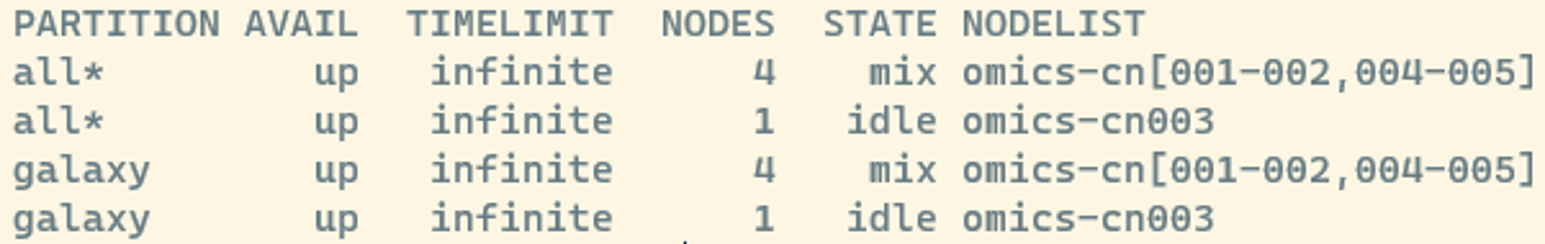
\includegraphics[width=0.6\textwidth,height=\textheight]{../img/sinfo.png}
\end{center}

Here, the different columns you see are:

\begin{itemize}
\tightlist
\item
  partition: tells us what queues that are available. There are few
  partitions on Crunchomics and you do not need to define them in our
  case. However, other systems use partitions to group a subset of nodes
  with different type of hardwares or a specific maximum wall time. For
  example, you might have specific partitions for memory-heavy versus
  time-intensive jobs.
\item
  state: tells you if a node is busy or not. Here:

  \begin{itemize}
  \tightlist
  \item
    mix : consumable resources partially allocated
  \item
    idle : available to requests consumable resources
  \item
    drain : unavailable for use per system administrator request
  \item
    alloc : consumable resources fully allocated
  \item
    down : unavailable for use.
  \end{itemize}
\item
  Nodes: The number of nodes available for each partition
\item
  NodeList: the names of the compute nodes (i.e.~omics-cn001 to
  omics-cn005)
\end{itemize}

\subsection{View info about jobs in the
queue}\label{view-info-about-jobs-in-the-queue}

The following command gives us some information about how busy the HPC
is:

\begin{Shaded}
\begin{Highlighting}[]
\ExtensionTok{squeue}
\end{Highlighting}
\end{Shaded}

After running this, you can see all jobs scheduled on the HPC, which
might look something like this:

\begin{center}
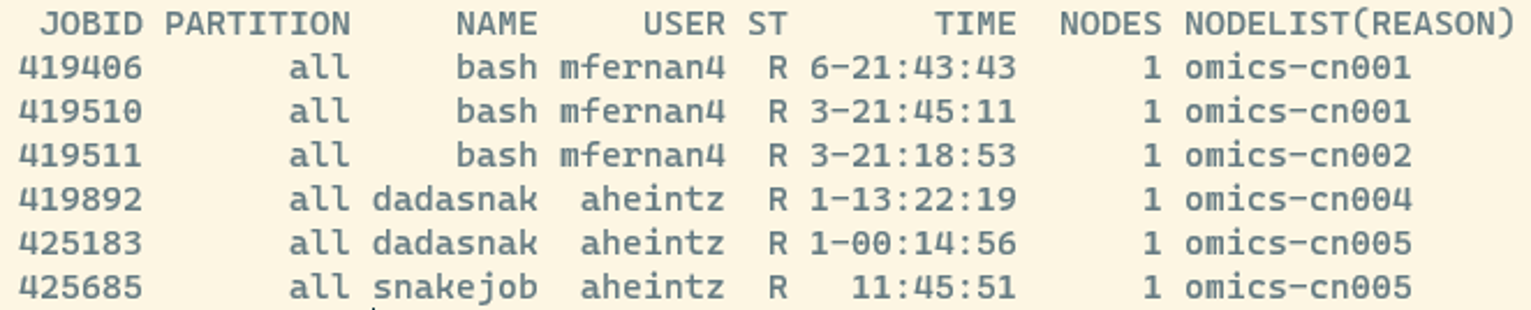
\includegraphics[width=0.5\textwidth,height=\textheight]{../img/squeue.png}
\end{center}

\begin{itemize}
\tightlist
\item
  JOBID: every job gets a number and you can manipulate jobs via this
  number
\item
  ST: Job state codes that describe the current state of the job. The
  full list of abbreviations can be found
  \href{https://curc.readthedocs.io/en/latest/running-jobs/squeue-status-codes.html}{here}
\end{itemize}

If we would have submitted a job, we also should see the job listed
there.

\section{\texorpdfstring{\texttt{srun}:Submitting a job
interactively}{srun:Submitting a job interactively}}\label{srunsubmitting-a-job-interactively}

\texttt{srun} is used when you want to run tasks interactively or want
to have more control over the execution of a job. You directly issue
\texttt{srun} commands in the terminal and you at the same time are able
to specify the tasks to be executed and their resource requirements. For
example, you might want to run softwareX and request that this job
requires 10 CPUs and 5 GB of memory.

Use \texttt{srun} when:

\begin{itemize}
\tightlist
\item
  You want to run tasks interactively and need immediate feedback
  printed to the screen
\item
  You are testing or debugging your commands before incorporating them
  into a script
\item
  You need more control over the execution of tasks
\item
  Typically, you use srun for smaller jobs that do not run for too long,
  i.e.~a few hours
\end{itemize}

Let's submit a very simple example for which we would not even need to
submit a job, but just to get you started.

\begin{Shaded}
\begin{Highlighting}[]
\ExtensionTok{srun}\NormalTok{ echo }\StringTok{"Hello interactively"}
\end{Highlighting}
\end{Shaded}

You should see the output of echo printed to the screen and if you would
run \texttt{squeue} you won't even see your job since everything ran so
fast. But congrats, you communicated the first time with the compute
node.

Now assume you want to run a more complex interactive task with
\texttt{srun} that might run longer and benefit from using more CPUs. In
this case you need to specify the resources your job needs by adding
flags, i.e.~some of which you see here:

\begin{Shaded}
\begin{Highlighting}[]
\ExtensionTok{srun} \AttributeTok{{-}{-}nodes}\OperatorTok{=}\NormalTok{1 }\AttributeTok{{-}{-}ntasks}\OperatorTok{=}\NormalTok{1 }\AttributeTok{{-}{-}cpus{-}per{-}task}\OperatorTok{=}\NormalTok{1 }\AttributeTok{{-}{-}mem}\OperatorTok{=}\NormalTok{1G echo }\StringTok{"Hello interactively"}
\end{Highlighting}
\end{Shaded}

The different flags mean the following:

\begin{itemize}
\tightlist
\item
  \texttt{-\/-nodes=1}: Specifies the number of nodes. In this case,
  it's set to 1 and tells slurm that we want to use a full node. Only
  use this if you make use of all resources on that node, otherwise
  omit. In our case this definitely is over-kill to request a full node
  with 64 CPUs to print a single line of text to the screen.
\item
  \texttt{-\/-ntasks=1}: Defines the number of tasks to run. Here, it's
  set to 1 since we want to use echo once
\item
  \texttt{-\/-cpus-per-task=1}: Specifies the number of CPUs per task.
  Adjust this based on the computational requirements of your task
\item
  \texttt{-\/-mem=1G}: Sets the memory requirement for the task. Modify
  this based on your task's memory needs
\item
  \texttt{echo\ "Hello\ interactively}: The actual command you want to
  run interactively
\end{itemize}

\subsection{Choosing the right amount of
resources}\label{choosing-the-right-amount-of-resources}

When you're just starting, deciding on the right resources to request
for your computational job can be a bit challenging. The resource
requirements can vary significantly based on the specific tool or
workflow you are using. Here are some general guidelines to help you
make informed choices:

\begin{itemize}
\tightlist
\item
  Use default settings: Begin by working with the default settings
  provided by the HPC cluster or recommended by the tool itself. These
  are often set to provide a balanced resource allocation for a wide
  range of tasks
\item
  Check the software documentation: Consult the documentation of the
  software or tool you are using. Many tools provide recommendations for
  resource allocation based on the nature of the computation.
\item
  Test with small datasets: For initial testing and debugging especially
  when working with large datasets, consider working with a smaller
  subset of your data. This allows for faster job turnaround times,
  helping you identify and resolve issues more efficiently.
\item
  Monitor the resources usage:

  \begin{itemize}
  \tightlist
  \item
    Use \texttt{sacct} to check what resources a finished job has used
    and see whether you can optimize a run if you plan to run similar
    jobs over and over again. An example command would be
    \texttt{sacct\ -j\ 419847\ -\/-format=User,JobID,Jobname,state,start,end,elapsed,MaxRss,ncpus.}
    In the report, look for columns like MaxRSS (maximum resident set
    size) to check if the amount of memory allocated (--mem) was
    appropriate.
  \item
    Ensuer that the job used the resources you requested. For instance,
    if you would have used \texttt{-\/-cpus-per-task=4\ -\/-mem=4G}, you
    would expect to use a total of 16 GB of memory (4 CPUs * 4 GB). You
    can verify this with \texttt{sacct} to ensure your job's resource
    requirements align with its actual usage.
  \end{itemize}
\item
  Fine-Tuning Resource Requests: If you encounter performance issues or
  your jobs are not completing successfully, consider iteratively
  adjusting resource requests. This might involve increasing or
  decreasing the number of CPUs, memory allocation, or other relevant
  parameters.
\end{itemize}

\subsection{Run FastQC with srun}\label{run-fastqc-with-srun}

\href{https://www.bioinformatics.babraham.ac.uk/projects/fastqc/}{FastQC}
is a quality control tool for high throughput sequence data that is
already installed on Crunchomics. This will be the actual software that
we now want to run to look more closely at the quality of the sequencing
data that we just uploaded to Crunchomics.

By the way: Whenever running a software for a first time, it is useful
to check the manual, for example with \texttt{fastqc\ -h.}

Let's start by setting up a clean folder structure to keep our files
organized. I start with making a folder in which I want to store all
results generated in this analysis and by using the \texttt{-p} argument
I generate a fastqc folder inside the results folder at the same time.
Then, we can submit our job using \texttt{srun}.

\begin{Shaded}
\begin{Highlighting}[]
\FunctionTok{mkdir} \AttributeTok{{-}p}\NormalTok{ results/fastqc }

\ExtensionTok{srun} \AttributeTok{{-}{-}cpus{-}per{-}task}\OperatorTok{=}\NormalTok{1 }\AttributeTok{{-}{-}mem}\OperatorTok{=}\NormalTok{5G fastqc data/seq\_project/}\PreprocessorTok{*}\NormalTok{/}\PreprocessorTok{*}\NormalTok{gz }\AttributeTok{{-}o}\NormalTok{ results/fastqc  }\AttributeTok{{-}{-}threads}\NormalTok{ 1}

\ExtensionTok{ll}\NormalTok{ results/fastqc/}\PreprocessorTok{*}
\end{Highlighting}
\end{Shaded}

Since we work with little data this will run extremely fast despite only
using 1 CPU (or thread, in our case these two words can be used
interchangeably). However, if you would be logged into Crunchomics via a
second window and run \texttt{squeue} you should see that your job is
actively running (in the example below, the job we submitted is named
after the software and got the jobid 746):

\begin{center}
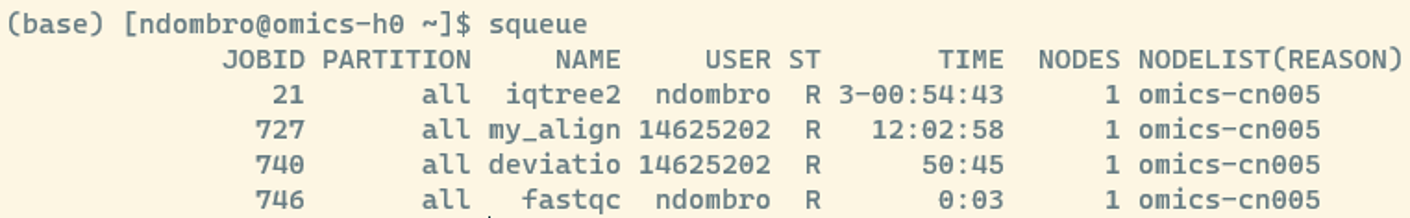
\includegraphics[width=0.5\textwidth,height=\textheight]{../img/squeue2.png}
\end{center}

Additionally, after the run is completed, you should see that several
HTML files were generated in our fastqc folder.

\begin{tcolorbox}[enhanced jigsaw, colframe=quarto-callout-caution-color-frame, breakable, opacityback=0, toptitle=1mm, left=2mm, coltitle=black, colbacktitle=quarto-callout-caution-color!10!white, title=\textcolor{quarto-callout-caution-color}{\faFire}\hspace{0.5em}{Exercise}, rightrule=.15mm, bottomtitle=1mm, titlerule=0mm, colback=white, arc=.35mm, toprule=.15mm, bottomrule=.15mm, leftrule=.75mm, opacitybacktitle=0.6]

Use scp to download the HTML files generated by fastqc to your own
computer and view one of the HTML files.

Click me to see an answer

\begin{Shaded}
\begin{Highlighting}[]
\FunctionTok{scp}\NormalTok{ username@omics{-}h0.science.uva.nl:/home/username/personal/projectX/results/fastqc/}\PreprocessorTok{*}\NormalTok{html results/fastqc/}
\end{Highlighting}
\end{Shaded}

You could also open a file on Crunchomics with
\texttt{firefox\ results/fastqc/Sample-DUMMY1\_R1\_fastqc.html}.
However, connecting to the internet via a cli on a remote server tends
to be rather slow and its often better to view files on your own
computer especially if they are large files.

If you want to know more about how to to interpret the output, you can
visit
\href{https://www.bioinformatics.babraham.ac.uk/projects/fastqc/}{the
fastqc website}, which gives some examples for interpreting good and bad
reports.

\end{tcolorbox}

\section{\texorpdfstring{\texttt{screen}: Submitting long running jobs
via
srun}{screen: Submitting long running jobs via srun}}\label{screen-submitting-long-running-jobs-via-srun}

One down-side of \texttt{srun} for long running jobs is that your
terminal gets ``blocked'' as long as the job is running and your job
will be aborted if you loose the ssh connection to the HPC. For long
running jobs, there are two ways to deal with this:

\begin{enumerate}
\def\labelenumi{\arabic{enumi}.}
\tightlist
\item
  submit a srun job in a screen
\item
  use sbatch
\end{enumerate}

In this section, we will cover how to use screen. Screen or GNU Screen
is a terminal multiplexer. This means that you can start a screen
session and then open any number of windows (virtual terminals) inside
that session.

Processes running in Screen will continue to run when their window is
not visible even if you get disconnected. This is perfect, if we start
longer running processes on the server and want to shut down our
computer when leaving for the day. As long as the server is still
connected to the internet, your process will continue running.

We start a screen as follows:

\begin{Shaded}
\begin{Highlighting}[]
\ExtensionTok{screen}
\end{Highlighting}
\end{Shaded}

We detach (go outside of a screen but keep the screen running in the
background) from a screen by pressing \texttt{control+a+d}.

If you want to run multiple analyses in multiple screens at the same
time, then can be useful to give your screens more descriptive names.
You can give screens a name using the \texttt{-S} option:

\begin{Shaded}
\begin{Highlighting}[]
\ExtensionTok{screen} \AttributeTok{{-}S}\NormalTok{ run\_fastqc}
\end{Highlighting}
\end{Shaded}

After detaching from this screen again with \texttt{control+a+d} you can
create a list of all currently running screens with:

\begin{Shaded}
\begin{Highlighting}[]
\ExtensionTok{screen} \AttributeTok{{-}ls}
\end{Highlighting}
\end{Shaded}

You can re-connect to an existing screen like this:

\begin{Shaded}
\begin{Highlighting}[]
\ExtensionTok{screen} \AttributeTok{{-}r}\NormalTok{ run\_fastqc}
\end{Highlighting}
\end{Shaded}

Now inside our screen, we can run fastqc same as we did before (but now
don't risk to loose a long-running job):

\begin{Shaded}
\begin{Highlighting}[]
\ExtensionTok{srun} \AttributeTok{{-}{-}cpus{-}per{-}task}\OperatorTok{=}\NormalTok{1 }\AttributeTok{{-}{-}mem}\OperatorTok{=}\NormalTok{5G fastqc data/seq\_project/}\PreprocessorTok{*}\NormalTok{/}\PreprocessorTok{*}\NormalTok{gz }\AttributeTok{{-}o}\NormalTok{ results/fastqc  }\AttributeTok{{-}{-}threads}\NormalTok{ 1 }
\end{Highlighting}
\end{Shaded}

For long-running jobs we can start multiple screens at once or even if
we just have one screen open, close it and leave for the day or simply
work on other things on the cli outside of the screen.

If you want to completely close and remove a screen, type the following
and press enter while being inside of the screen:

\begin{Shaded}
\begin{Highlighting}[]
\BuiltInTok{exit}
\end{Highlighting}
\end{Shaded}

\section{\texorpdfstring{\texttt{sbatch}: submitting a long-running
job}{sbatch: submitting a long-running job}}\label{sbatch-submitting-a-long-running-job}

\texttt{sbatch} is your go-to command when you have a script (i.e.~a
batch script) that needs to be executed without direct user interaction.

Use \texttt{sbatch} when:

\begin{itemize}
\tightlist
\item
  You have long-running or resource-intensive tasks
\item
  You want to submit jobs that can run independently without your
  immediate supervision
\item
  You want to submit multiple jobs at once
\end{itemize}

To run a job script, you:

\begin{itemize}
\tightlist
\item
  create a script that contains all the commands and configurations
  needed for your job
\item
  use sbatch to submit this script to the Slurm scheduler, and it takes
  care of the rest.
\end{itemize}

Let's start with generating some new folders to keep our project folder
organized:

\begin{Shaded}
\begin{Highlighting}[]
\FunctionTok{mkdir}\NormalTok{ scripts }
\FunctionTok{mkdir}\NormalTok{ logs}
\end{Highlighting}
\end{Shaded}

To get started, assume we have created a script in the scripts folder
named \texttt{run\_fastqc.sh} with the content that is shown below.
Notice, how in this script I added some additional \texttt{echo}
commands? I just use these to print some information about the progress
which could be printed to a log file but if you have several commands
that should be executed after each other that is how you would do it.

\begin{Shaded}
\begin{Highlighting}[]
\CommentTok{\#!/bin/bash}
\CommentTok{\#SBATCH {-}{-}cpus{-}per{-}task=1}
\CommentTok{\#SBATCH {-}{-}mem=5G}

\BuiltInTok{echo} \StringTok{"Start fastqc"}

\ExtensionTok{fastqc}\NormalTok{ data/seq\_project/}\PreprocessorTok{*}\NormalTok{/}\PreprocessorTok{*}\NormalTok{gz }\AttributeTok{{-}o}\NormalTok{ results/fastqc  }\AttributeTok{{-}{-}threads}\NormalTok{ 1}

\BuiltInTok{echo} \StringTok{"fastqc finished"}
\end{Highlighting}
\end{Shaded}

In the job script above:

\begin{itemize}
\tightlist
\item
  \texttt{\#!/bin/bash} . This so-called Shebang line tells the shell to
  interpret and run the Slurm script using the bash shell.~This line
  should always be added at the very top of your SBATCH/Slurm script.
\item
  The lines that follow and start with \texttt{\#} are the lines in
  which we define the amount of resources required for our job to run.
  In our case, we request 1 CPU and 5G of memory.
\item
  If your code needs any dependencies, such as conda environments, you
  would add these dependencies here. We do not need this for our example
  here, but you might need to add something like this
  \texttt{conda\ activate\ my\_env} if you have installed your own
  software. We will touch upon conda environments and installing
  software a bit later.
\item
  The lines afterwards are the actually commands that we want to run on
  the compute nodes, We also call this the job steps.
\end{itemize}

To prepare the script and run it:

\begin{itemize}
\tightlist
\item
  Run \texttt{nano\ scripts/run\_fastqc.sh} to generate an empty
  jobscript file
\item
  Add the code from above into the file we just opened
\item
  Press \texttt{ctrl+x} to exit nano
\item
  Type \texttt{Y} when prompted if the changes should be saved
\item
  Confirm that the file name is good by pressing enter
\end{itemize}

Afterwards, you can submit \texttt{run\_fastqc.sh} as follows:

\begin{Shaded}
\begin{Highlighting}[]
\CommentTok{\#submit job: 754}
\ExtensionTok{sbatch}\NormalTok{ scripts/run\_fastqc.sh}

\CommentTok{\#check if job is running correctly}
\ExtensionTok{squeue}
\end{Highlighting}
\end{Shaded}

After running this, you should see that the job was submitted and
something like this printed to the screen
\texttt{Submitted\ batch\ job\ 754}. You will also see that a new file
is generated that will look something like this \texttt{slurm-754.out}.

When you submit a batch job using sbatch, Slurm redirects the standard
output and standard error messages, which you have seen printed to the
screen when you used \texttt{srun}, to a file named in the format
slurm-JOBID.out, where JOBID is the unique identifier assigned to your
job.

This file is useful as it:

\begin{itemize}
\tightlist
\item
  Captures the output of our batch scripts and stores them in a file
\item
  Can be used for debugging, since if something goes wrong with your
  job, examining the contents of this file can provide valuable insights
  into the issue. Error messages, warnings, or unexpected outputs are
  often recorded here
\end{itemize}

Feel free to explore the content of the log file, do you see how the
echo commands are used as well?

\begin{tcolorbox}[enhanced jigsaw, colframe=quarto-callout-tip-color-frame, breakable, opacityback=0, toptitle=1mm, left=2mm, coltitle=black, colbacktitle=quarto-callout-tip-color!10!white, title=\textcolor{quarto-callout-tip-color}{\faLightbulb}\hspace{0.5em}{Tip: sbatch and better log files}, rightrule=.15mm, bottomtitle=1mm, titlerule=0mm, colback=white, arc=.35mm, toprule=.15mm, bottomrule=.15mm, leftrule=.75mm, opacitybacktitle=0.6]

We have seen that by default \texttt{sbatch} redirects the standard
output and error to our working directory and that it decides itself how
to name the files. Since file organization is very important especially
if you generate lots of files, you find below an example to:

\begin{itemize}
\tightlist
\item
  Store the standard output and error in two separate files
\item
  Redirect the output into another folder, the logs folder
\item
  In the code below, the \texttt{\%j} is replaced with the job
  allocation number once the log files are generated
\end{itemize}

\begin{Shaded}
\begin{Highlighting}[]
\CommentTok{\#!/bin/bash}
\CommentTok{\#SBATCH {-}{-}job{-}name=our\_fastqc\_job}
\CommentTok{\#SBATCH {-}{-}output=logs/fastqc\_\%j.out}
\CommentTok{\#SBATCH {-}{-}error=logs/fastqc\_\%j.err}
\CommentTok{\#SBATCH {-}{-}cpus{-}per{-}task=1}
\CommentTok{\#SBATCH {-}{-}mem=5G}

\BuiltInTok{echo} \StringTok{"Start fastqc"}

\ExtensionTok{fastqc}\NormalTok{ data/seq\_project/}\PreprocessorTok{*}\NormalTok{/}\PreprocessorTok{*}\NormalTok{gz }\AttributeTok{{-}o}\NormalTok{ results/fastqc  }\AttributeTok{{-}{-}threads}\NormalTok{ 1}

\BuiltInTok{echo} \StringTok{"fastqc finished"}
\end{Highlighting}
\end{Shaded}

\end{tcolorbox}

\begin{tcolorbox}[enhanced jigsaw, colframe=quarto-callout-tip-color-frame, breakable, opacityback=0, toptitle=1mm, left=2mm, coltitle=black, colbacktitle=quarto-callout-tip-color!10!white, title=\textcolor{quarto-callout-tip-color}{\faLightbulb}\hspace{0.5em}{Advanced tip: sbatch arrays to run multiple files in parallel}, rightrule=.15mm, bottomtitle=1mm, titlerule=0mm, colback=white, arc=.35mm, toprule=.15mm, bottomrule=.15mm, leftrule=.75mm, opacitybacktitle=0.6]

With fastqc we are very lucky that the tool can identify all the fastq
files in the directory we specify with \texttt{-o} by making use of the
wildcard. This is extremely useful for us but by far not all programs
work this way.

For this section, lets assume that we need to provide each individual
file we want to analyse, one by one, and can not provide a folder name.
How would we run such a job effectively?

What we want to do is created what is called a job array that allows us
to:

\begin{itemize}
\tightlist
\item
  Run multiple jobs that have the same job definition, i.e.~cpus, memory
  and software used
\item
  Run these job in the most optimal way. I.e. we do not want to run one
  job after each other but we also want to run jobs in parallel at the
  same time to optimize resource usage.
\end{itemize}

Let's start with making a list with files we want to work with based on
what we have already learned:

\begin{Shaded}
\begin{Highlighting}[]
\FunctionTok{ls}\NormalTok{ data/seq\_project/}\PreprocessorTok{*}\NormalTok{/}\PreprocessorTok{*}\NormalTok{.gz }\KeywordTok{|} \FunctionTok{cut} \AttributeTok{{-}f4} \AttributeTok{{-}d} \StringTok{"/"} \OperatorTok{\textgreater{}}\NormalTok{ samples.txt}
\end{Highlighting}
\end{Shaded}

Next, we can use this text file in our job array, the content of which
we store in \texttt{scripts/array.sh}:

\begin{Shaded}
\begin{Highlighting}[]
\CommentTok{\#!/bin/bash}

\CommentTok{\#SBATCH {-}{-}job{-}name=my\_array}
\CommentTok{\#SBATCH {-}{-}output=logs/array\_\%A\_\%a.out}
\CommentTok{\#SBATCH {-}{-}error=logs/array\_\%A\_\%a.err}
\CommentTok{\#SBATCH {-}{-}array=1{-}8}
\CommentTok{\#SBATCH {-}{-}cpus{-}per{-}task=1}
\CommentTok{\#SBATCH {-}{-}mem{-}per{-}cpu=5G}

\CommentTok{\#calculate the index of the current job within the batch}
\CommentTok{\#in our case the index will store the values 1 to 8 for our 8 files}
\VariableTok{INDEX}\OperatorTok{=}\VariableTok{$((SLURM\_ARRAY\_TASK\_ID} \VariableTok{))}

\CommentTok{\#build an array structure that stores the fastq.gz file names}
\VariableTok{CURRENT\_SAMPLE}\OperatorTok{=}\VariableTok{$(}\FunctionTok{cat}\NormalTok{ samples.txt }\KeywordTok{|}  \FunctionTok{sed} \AttributeTok{{-}n} \StringTok{"}\VariableTok{$\{INDEX\}}\StringTok{p"}\VariableTok{)}

\CommentTok{\#print what is actually happening}
\BuiltInTok{echo} \StringTok{"Now Job}\VariableTok{$\{INDEX\}}\StringTok{ runs on }\VariableTok{$\{CURRENT\_SAMPLE\}}\StringTok{"}

\CommentTok{\#run the actual job}
\ExtensionTok{fastqc}\NormalTok{ data/seq\_project/}\PreprocessorTok{*}\NormalTok{/}\VariableTok{$\{CURRENT\_SAMPLE\}} \AttributeTok{{-}o}\NormalTok{ results/fastqc  }\AttributeTok{{-}{-}threads}\NormalTok{ 1}
\end{Highlighting}
\end{Shaded}

In the script we use some new SLURM arguments:

\begin{itemize}
\tightlist
\item
  \texttt{\#SBATCH\ -\/-array=1-8}: Sets up a job array, specifying the
  range (1-8). We choose 1-8 because we have exactly 8 fastq.gz files we
  want to analyse
\item
  \texttt{\#SBATCH\ -\/-output=logs/array\_\%A\_\%a.out}: Store the
  standard output and error. \texttt{\%A} represents the job ID assigned
  by Slurm, and \texttt{\%a} represents the array task ID
\item
  \textbf{Important}: Are your individual arrays large jobs that use a
  lot of CPUs/memory? Then you might not want to submit all at the same
  time but submit them in a step-wise manner. With
  \texttt{\#SBATCH\ -\/-array=1-8\%2} you would only submit the first
  two jobs and only after these have finished the next jobs. Remember,
  try to use not more than \textasciitilde20\% of the crunchomics
  cluster at the same time.
\end{itemize}

The job does the following:

\begin{itemize}
\tightlist
\item
  The \texttt{INDEX} variable is storing the value of the current
  \texttt{SLURM\_ARRAY\_TASK\_ID}. This represents the ID of the current
  job within the array. In our case this will be first 1, then 2,
  \ldots, and finally 8.
\item
  Next, we build the array structure in which the
  \texttt{CURRENT\_SAMPLE} variable is created by:

  \begin{itemize}
  \tightlist
  \item
    Reading the \texttt{sample\_list.txt} file with \texttt{cat}
  \item
    Using a pipe to extract the file name at the calculated index using
    sed.
    \href{https://scienceparkstudygroup.github.io/software_information/source/cli/cli_file_manipulation.html\#sed-manipulating-the-content-of-files}{Sed}
    is an extremely powerful way to edit text that we have not covered
    here but \texttt{-n\ 1p} is a option that allows us to print one
    specific line of a file, in our case the first one when running
    array 1. So for the first array the actual code run is the following
    \texttt{cat\ samples.txt\ \textbar{}\ \ sed\ -n\ "1p"}. For the next
    array, we would run
    \texttt{cat\ samples.txt\ \textbar{}\ \ sed\ -n\ "2p"} and so forth.
  \item
    The output of the pipe is stored in a variable, called
    \texttt{CURRENT\_SAMPLE}. For our first sample this will be
    \texttt{Sample-DUMMY1\_R1.fastq.gz}
  \end{itemize}
\item
  We use echo to record what was executed when and store this
  information in the standard output
\item
  We run our actual fastqc job on the file name that is currently stored
  in the \texttt{CURRENT\_SAMPLE} variable.
\end{itemize}

If we check what is happening right after submitting the job with
\texttt{squeue} we should see something like this:

\begin{center}
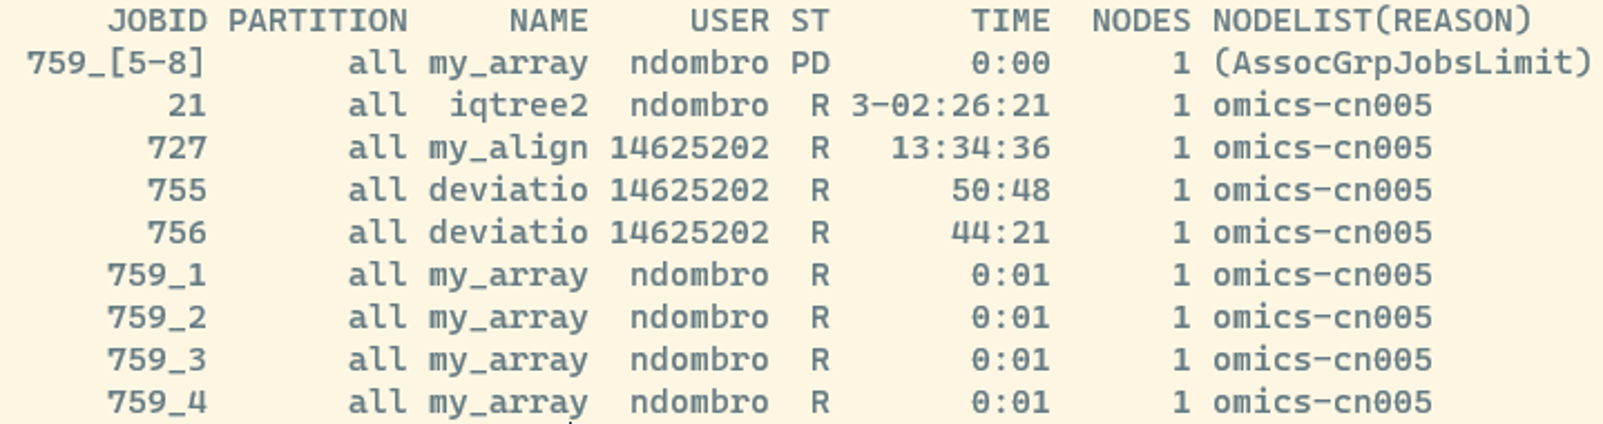
\includegraphics[width=0.5\textwidth,height=\textheight]{../img/arrays.png}
\end{center}

We see that jobs 1-4 are already running and the jobs 5-8 are currently
waiting for space. That is one of the useful things using a job manager
such as SLURM. It takes care of finding the appropriate resources on all
nodes for us as long as we defined the required cpus and memory
sensibly.

If we check the log files we should see something like this:

\begin{center}
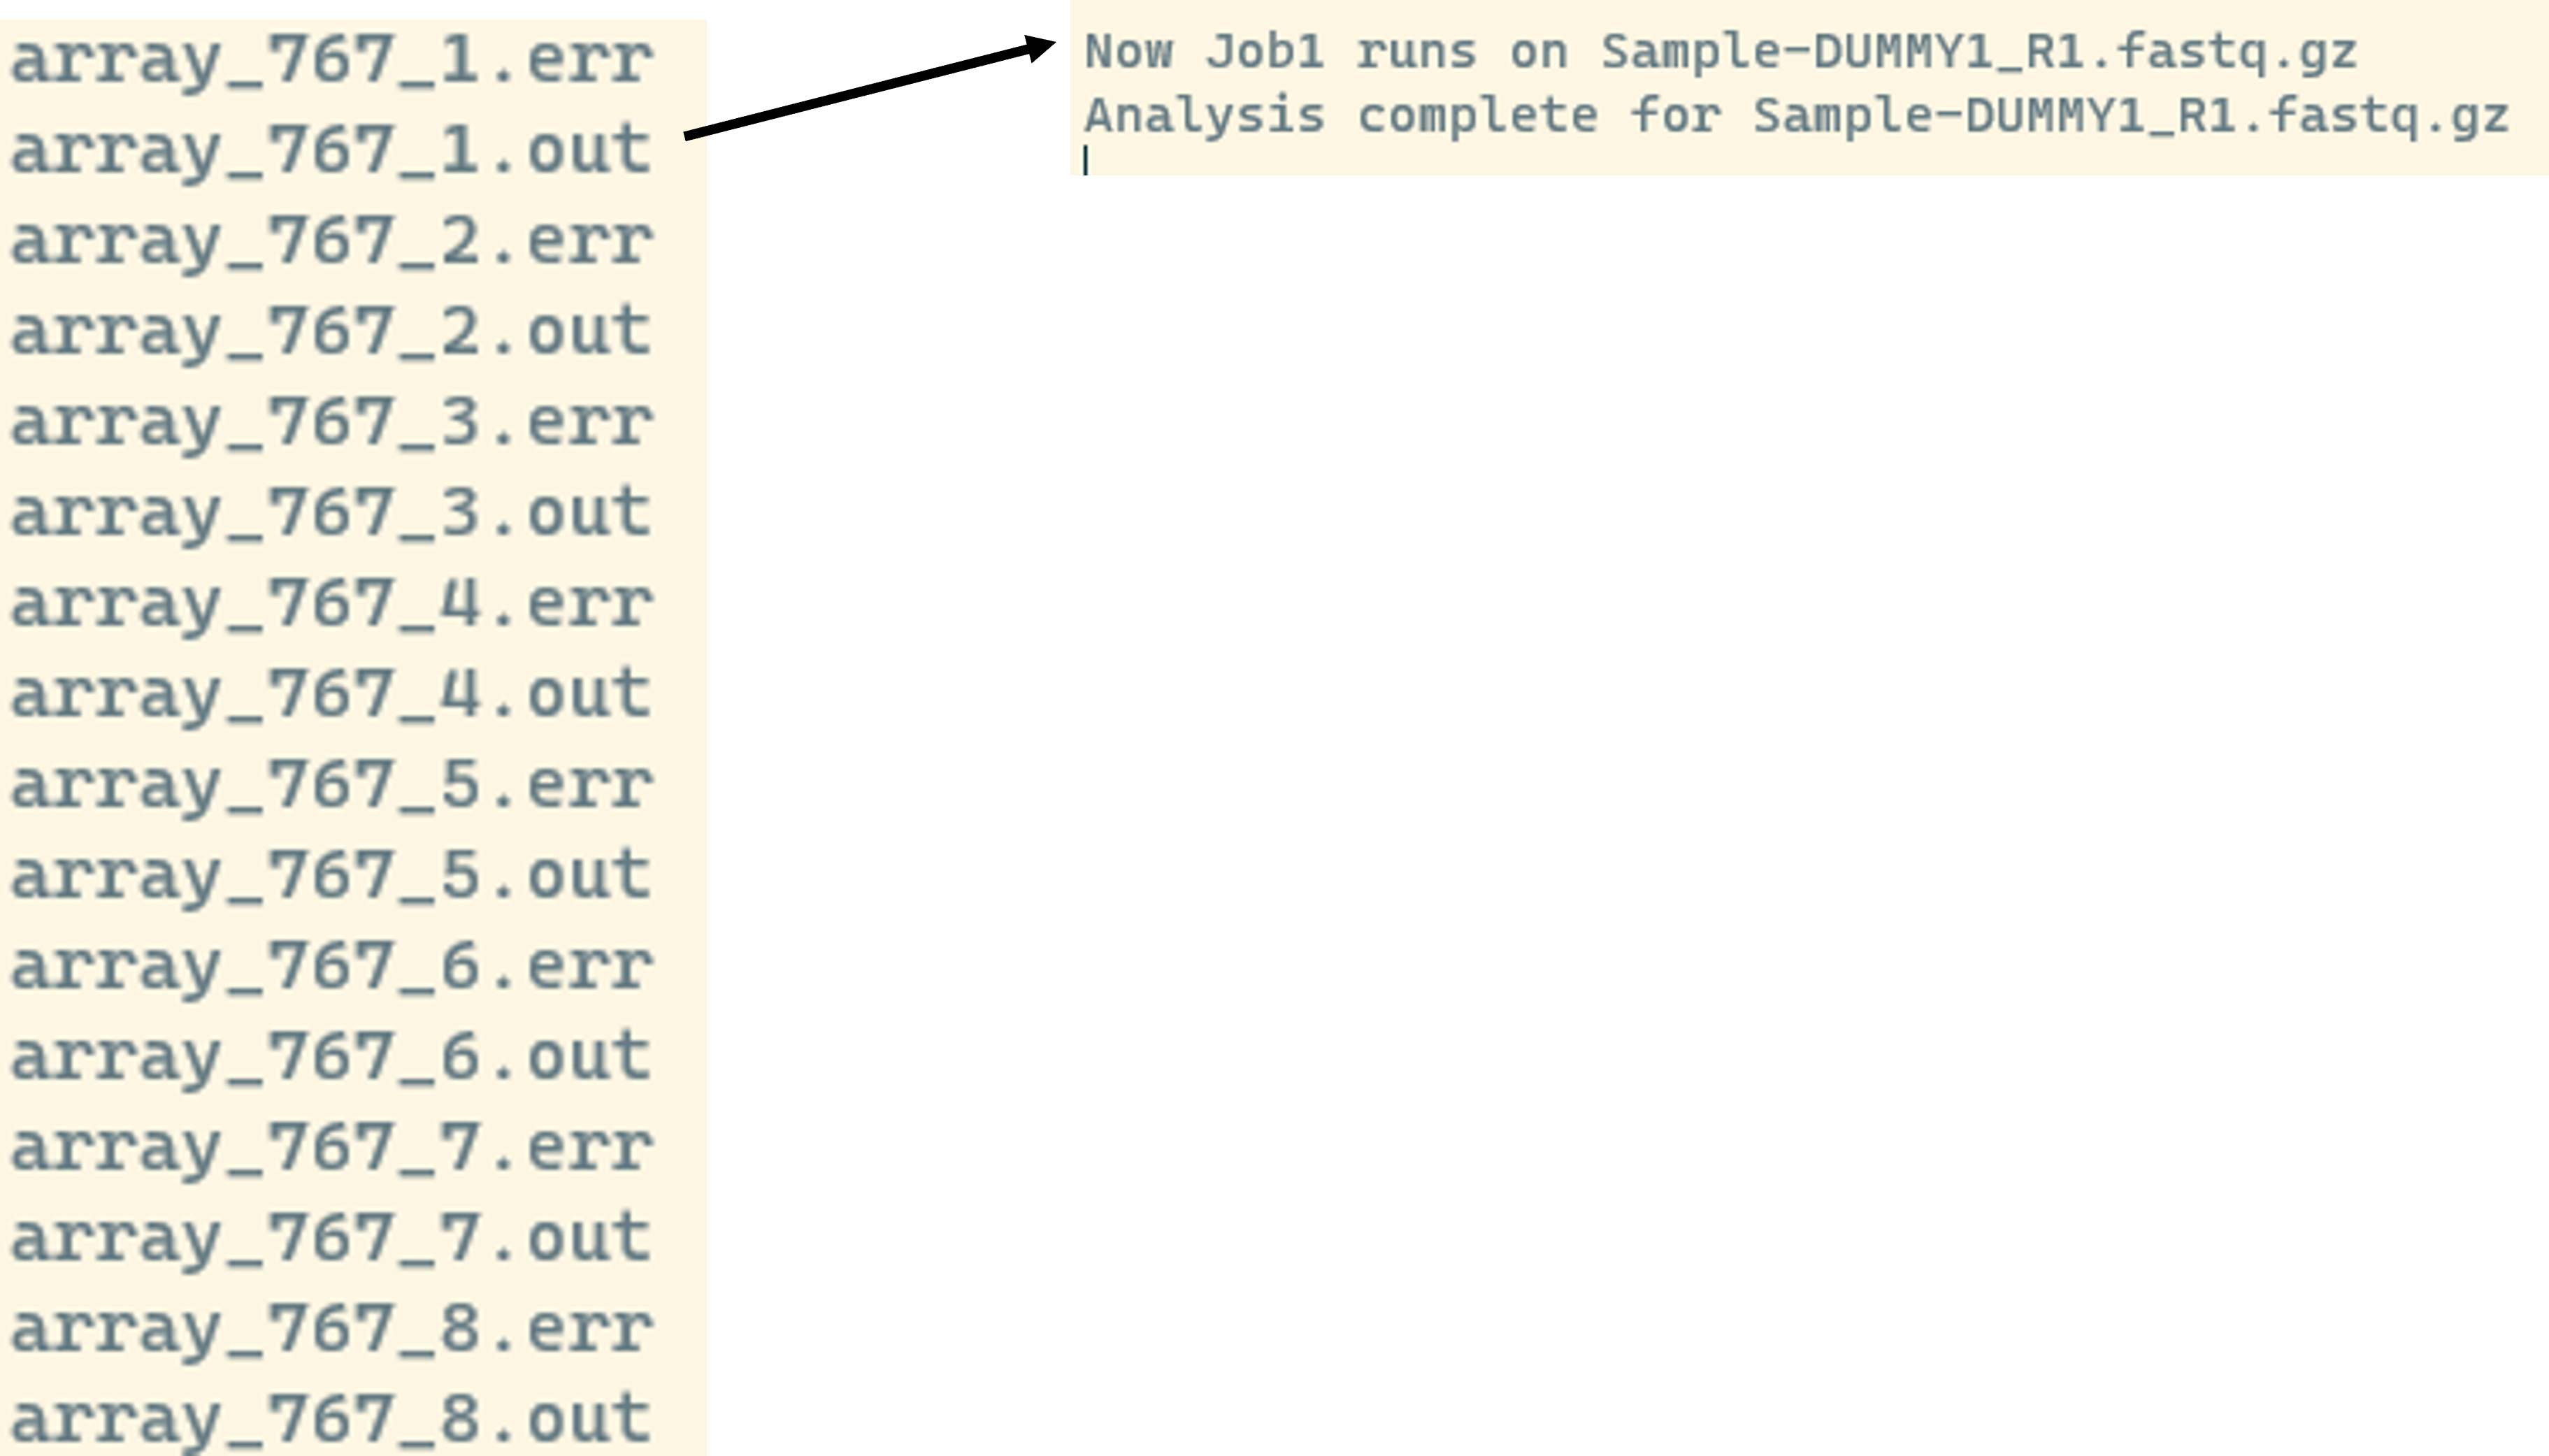
\includegraphics[width=0.5\textwidth,height=\textheight]{../img/arrays2.png}
\end{center}

We see that we get an individual output and error file for each job. In
the output we see what value is stored in the \texttt{INDEX}, here 1,
and the \texttt{CURRENT\_SAMPLE}, here
\texttt{Sample-DUMMY1\_R1.fastq.gz} and that the analysis finished
successfully.

\end{tcolorbox}

\section{Installing software}\label{installing-software}

There might be cases where the software you are interested in is not
installed on the HPC you are working with (or on your own computer).

In the majority of cases, you should be able to install software by
using a package management system, such as conda or mamba. These systems
allow you to find and install packages in their own environment without
administrator privileges. Let's have a look at a very brief example:

\subsection{Install conda/mamba}\label{install-condamamba}

A lot of systems already come with conda/mamba installed, however, if
possible we recommend working with mamba instead of conda. mamba is a
replacement and uses the same commands and configuration options as
conda, however, it tends to be much faster. A useful thing is that if
you find documentation for conda then you can swap almost all commands
between conda \& mamba.

If you have conda installed and do not want to install anything else,
that is fine. Just replace all instances of mamba with conda below.

This command should work in most cases to setup conda together with
mamba:

\begin{Shaded}
\begin{Highlighting}[]
\ExtensionTok{curl} \AttributeTok{{-}L} \AttributeTok{{-}O} \StringTok{"https://github.com/conda{-}forge/miniforge/releases/latest/download/Miniforge3{-}}\VariableTok{$(}\FunctionTok{uname}\VariableTok{)}\StringTok{{-}}\VariableTok{$(}\FunctionTok{uname} \AttributeTok{{-}m}\VariableTok{)}\StringTok{.sh"}
\FunctionTok{bash}\NormalTok{ Miniforge3{-}}\VariableTok{$(}\FunctionTok{uname}\VariableTok{)}\NormalTok{{-}}\VariableTok{$(}\FunctionTok{uname} \AttributeTok{{-}m}\VariableTok{)}\NormalTok{.sh}
\end{Highlighting}
\end{Shaded}

\subsection{Setting up an environment}\label{setting-up-an-environment}

Let's assume we want to install seqkit, a tool that allows us to
calculate some statistics for sequencing data such as the number of
sequences or average sequence length per sample.

We can install seqkit into a separate environment, which we can give a
descriptive name, as follows:

\begin{Shaded}
\begin{Highlighting}[]
\CommentTok{\#check if the tool is installed (should return "command not" found if the software is not installed)}
\ExtensionTok{seqkit} \AttributeTok{{-}h}

\CommentTok{\#create an empty environment and name it seqkit and we add the version number to the name}
\CommentTok{\#this basically sets up seqkit separate from our default working environment}
\CommentTok{\#this is useful whenever software require complicated dependencies allowing us to have a separate install away from software that could conflict with each other}
\ExtensionTok{mamba}\NormalTok{ create }\AttributeTok{{-}n}\NormalTok{ seqkit\_2.6.1}

\CommentTok{\#install seqkit, into the environment we just created}
\ExtensionTok{mamba}\NormalTok{ install }\AttributeTok{{-}n}\NormalTok{ seqkit\_2.6.1 }\AttributeTok{{-}c}\NormalTok{ bioconda seqkit=2.6.1}

\CommentTok{\#to run seqkit, we need activate the environment first}
\ExtensionTok{mamba}\NormalTok{ activate seqkit\_2.6.1}

\CommentTok{\#check if tool is installed, }
\CommentTok{\#if installed properly this should return some detailed information on how to run seqkit}
\ExtensionTok{seqkit} \AttributeTok{{-}h}

\CommentTok{\#run the tool via srun}
\FunctionTok{mkdir}\NormalTok{ results/seqkit}
\ExtensionTok{srun} \AttributeTok{{-}{-}cpus{-}per{-}task}\NormalTok{ 2 }\AttributeTok{{-}{-}mem}\OperatorTok{=}\NormalTok{4G seqkit stats }\AttributeTok{{-}a} \AttributeTok{{-}To}\NormalTok{ results/seqkit/seqkit\_stats.tsv data/seq\_project/}\PreprocessorTok{*}\NormalTok{/}\PreprocessorTok{*}\NormalTok{.gz }\AttributeTok{{-}{-}threads}\NormalTok{ 2}
\FunctionTok{less} \AttributeTok{{-}S}\NormalTok{ results/seqkit/seqkit\_stats.tsv }

\CommentTok{\#close the environment}
\ExtensionTok{conda}\NormalTok{ deactivate}
\end{Highlighting}
\end{Shaded}

When installing seqkit, we:

\begin{itemize}
\tightlist
\item
  specify the exact version we want to download with \texttt{=2.6.1}. We
  could also install the newest version that conda/mamba can find by
  running \texttt{mamba\ install\ -n\ seqkit\ -c\ bioconda\ seqkit}.
\item
  specify that we want to look for seqkit in the bioconda channel with
  the option \texttt{-c}. Channels are the locations where packages are
  stored. They serve as the base for hosting and managing packages.
  Conda packages are downloaded from remote channels, which are URLs to
  directories containing conda packages. If you are unable to find a
  package it might be that you need to specify a channel.
\end{itemize}

Forgot what conda environments you installed in the past? You can run
\texttt{conda\ env\ list} to generate a list of all existing
environments.

Unsure if a software can be installed with conda? Google conda together
with the software name, which should lead you do a conda web page. This
page should inform you whether you need to add a specific channel to
install the software as well as the version numbers available.

A full set of mamba/conda commands can be found
\href{https://docs.conda.io/projects/conda/en/latest/commands/index.html.}{here}.

\begin{tcolorbox}[enhanced jigsaw, colframe=quarto-callout-caution-color-frame, breakable, opacityback=0, toptitle=1mm, left=2mm, coltitle=black, colbacktitle=quarto-callout-caution-color!10!white, title=\textcolor{quarto-callout-caution-color}{\faFire}\hspace{0.5em}{Exercise}, rightrule=.15mm, bottomtitle=1mm, titlerule=0mm, colback=white, arc=.35mm, toprule=.15mm, bottomrule=.15mm, leftrule=.75mm, opacitybacktitle=0.6]

\begin{enumerate}
\def\labelenumi{\arabic{enumi}.}
\tightlist
\item
  Download and view the file \texttt{results/seqkit/seqkit\_stats.tsv}
  on your own computer
\item
  Run the seqkit again but this time submit the job via a sbatch script
  instead of using srun. Notice, that you need to tell SLURM how it can
  activate the conda environment that has seqkit installed. You might
  need to google how to do that, since this requires some extra line of
  code that we have not covered yet but see this as a good exercise for
  how to handle error messages that you see in the log files for your
  own analyses
\end{enumerate}

Click me to see an answer

\begin{Shaded}
\begin{Highlighting}[]
\CommentTok{\#question 1}
\FunctionTok{scp}\NormalTok{ username@omics{-}h0.science.uva.nl:/home/ndombro/personal/projectX/results/seqkit/seqkit\_stats.tsv .}

\CommentTok{\#question 2 }
\ExtensionTok{sbatch}\NormalTok{ scripts/seqkit.sh}
\end{Highlighting}
\end{Shaded}

Content of \texttt{scripts/seqkit.sh}:

\begin{Shaded}
\begin{Highlighting}[]
\CommentTok{\#!/bin/bash}
\CommentTok{\#SBATCH {-}{-}job{-}name=seqkit\_job}
\CommentTok{\#SBATCH {-}{-}output=logs/seqkit\_\%j.out}
\CommentTok{\#SBATCH {-}{-}error=logs/seqkit\_\%j.err}
\CommentTok{\#SBATCH {-}{-}cpus{-}per{-}task=2}
\CommentTok{\#SBATCH {-}{-}mem=5G}

\CommentTok{\#activate dependencies}
\BuiltInTok{source}\NormalTok{ \textasciitilde{}/.bashrc}
\ExtensionTok{mamba}\NormalTok{ activate seqkit\_2.6.1}

\CommentTok{\#run seqkit}
\BuiltInTok{echo} \StringTok{"Start seqkit"}

\ExtensionTok{seqkit}\NormalTok{ stats }\AttributeTok{{-}a} \AttributeTok{{-}To}\NormalTok{ results/seqkit/seqkit\_stats.tsv data/seq\_project/}\PreprocessorTok{*}\NormalTok{/}\PreprocessorTok{*}\NormalTok{.gz }\AttributeTok{{-}{-}threads}\NormalTok{ 2}

\BuiltInTok{echo} \StringTok{"seqkit finished"}
\end{Highlighting}
\end{Shaded}

In the script above, we see that we need to add two lines of code to
activate the seqkit conda environment:

\begin{verbatim}
source ~/.bashrc
mamba activate seqkit_2.6.1
\end{verbatim}

When you run a script or a command, it operates in its own environment.
The source command is like telling the script to look into another file,
in this case, \texttt{\textasciitilde{}/.bashrc}, and execute the
commands in that file as if they were written directly into the script.

Here, \texttt{source\ \textasciitilde{}/.bashrc} is telling the script
to execute the commands in the \texttt{\textasciitilde{}/.bashrc} file.
This is typically done to set up environment variables, paths, and
activate any software or tools that are required for the script to run
successfully. In our case this tells Slurm where we have installed conda
and thus enables Slurm to use conda itself.

This allows slurm to, after executing
\texttt{source\ \textasciitilde{}/.bashrc}, activates a Conda
environment using \texttt{mamba\ activate\ seqkit\_2.6.1}. This ensures
that the SeqKit tool and its dependencies are available and properly
configured for use in the subsequent part of the script.

\end{tcolorbox}



\end{document}
